% Symmetry in AlphaFold 2: what the Supplementary Information proves, with figures.
% A note for the two presenters. Build: latexmk -pdf SYMMETRY.tex
\documentclass[10pt,a4paper]{article}
\usepackage[margin=18mm]{geometry}
\usepackage[T1]{fontenc}
\usepackage{XCharter}
\usepackage[xcharter,vvarbb]{newtxmath}
\usepackage{amsmath,bm,booktabs,microtype,xcolor,graphicx,tikz}
\usetikzlibrary{arrows.meta,calc,positioning}
\usepackage[colorlinks,allcolors=black]{hyperref}
\definecolor{ETHBlue}{RGB}{33,92,175}
\definecolor{ETHRed}{RGB}{183,53,45}
\definecolor{ETHGray}{RGB}{111,111,111}
\colorlet{evita}{ETHBlue}
\colorlet{ben}{ETHRed}
\setlength{\parindent}{0pt}
\setlength{\parskip}{4pt}
% Section titles carry the colour of the presenter whose slides the section belongs to.
\newcommand{\sect}[2]{\vspace{5pt}{\large\bfseries\color{#1}#2}\par\vspace{1pt}}
\newcommand{\SE}{\mathrm{SE}(3)}
\newcommand{\E}{\mathrm{E}(3)}
\newcommand{\vx}{\vec{\mathbf x}}
\newcommand{\vt}{\vec{\mathbf t}}
\newcommand{\vq}{\vec{\mathbf q}}
\newcommand{\vk}{\vec{\mathbf k}}
\newcommand{\vpt}{\vec{\mathbf v}}
\newcommand{\Tg}{T_{\text{global}}}
\newcommand{\si}[1]{\ifmmode\text{\footnotesize\textcolor{black!55}{(#1)}}\else{\footnotesize\textcolor{black!55}{(#1)}}\fi}
\newcommand{\figcap}[1]{\par\vspace{2pt}{\footnotesize\color{black!70}#1\par}}
% Drawings, in the style of the slides. All figures are illustrations, not data.
\tikzset{every node/.append style={execute at begin node=\sffamily\small}}
\newcommand{\frameaxes}[2]{%
  \draw[ETHRed, line width=1.2pt, -{Latex[length=4pt]}] #1 -- ++(#2:0.75);
  \draw[ETHRed, line width=1.2pt, -{Latex[length=4pt]}] #1 -- ++(#2+90:0.75);
  \fill[ETHRed] #1 circle (2.2pt);
}
\newcommand{\ipapair}{%
  \foreach \q/\k in {{(1.0,0.9)}/{(2.5,1.0)}, {(1.3,0.3)}/{(2.25,0.4)}, {(1.2,-0.3)}/{(2.4,-0.25)}, {(0.85,-0.85)}/{(2.65,-0.8)}} {
    \draw[ETHBlue!45, line width=0.6pt] (0,0) -- \q;
    \draw[black!40, line width=0.6pt] (3.6,0.1) -- \k;
    \draw[ETHRed, line width=0.9pt, densely dashed] \q -- \k;
    \fill[ETHBlue] \q circle (2.2pt);
    \fill[black] \k circle (2.2pt);
  }
  \frameaxes{(0,0)}{115}
  \frameaxes{(3.6,0.1)}{-25}
}
\newcommand{\fapechain}[4]{% colour, atom i-1, atom i, label shift
  \draw[#1!45, line width=1.2pt, line cap=round, line join=round]
    (0,0) -- (0.8,0.5) -- (1.6,0.1) -- (2.3,0.8) -- #2 -- #3;
  \foreach \p in {(0,0), (0.8,0.5), (2.3,0.8), #2} \fill[#1!45] \p circle (2pt);
  \frameaxes{(1.6,0.1)}{45}
  \draw[#1, line width=1.2pt, -{Latex[length=4.5pt]}, shorten >=2.4pt] (1.6,0.1) -- #3;
  \fill[#1] #3 circle (2.6pt);
  \node[text=#1] at #3 [shift={#4}] {$i$};
}
% A point above (odot) or below (otimes) the page
\newcommand{\abovepage}[1]{\draw[line width=0.9pt] #1 circle (3.2pt); \fill #1 circle (1.1pt);}
\newcommand{\belowpage}[1]{\draw[line width=0.9pt] #1 circle (3.2pt); \draw[line width=0.9pt] ($#1+(-2.1pt,-2.1pt)$) -- ($#1+(2.1pt,2.1pt)$) ($#1+(-2.1pt,2.1pt)$) -- ($#1+(2.1pt,-2.1pt)$);}

\begin{document}

{\LARGE\bfseries Symmetry in the structure module and the loss\par}
\vspace{2pt}
{\large What the Supplementary Information of Jumper et al.\ (2021) proves, and what it does not claim\par}
\vspace{4pt}
Equations are from the SI, with section and equation numbers in grey, pages are printed pages. Drawings are illustrations.
Headings in \textcolor{evita}{blue} belong to Evita's slides 10 and 11, in \textcolor{ben}{red} to the FAPE slide 12. Black is shared ground.

\sect{black}{0. Notation and the one definition that matters \si{SI 1.1, 1.8, 1.8.2}}
A frame is a Euclidean transform $T=(R,\vt)$. It maps local to global coordinates and composes as
\[
T\circ\vx = R\vx+\vt, \qquad
(R_1,\vt_1)\circ(R_2,\vt_2) = (R_1R_2,\; R_1\vt_2+\vt_1). \qquad\si{SI 1.1}
\]
The SI never names a group. It defines the word it uses instead: ``rigid motion'' includes proper rotation and translation but not reflection \si{SI 1.8.2, p.~28}. In group language a rigid motion is an element of $\SE$, $\det R=+1$. The larger group $\E$ also contains reflections, $\det R=-1$. Every claim below is about $\SE$. Reflections are treated separately, because the paper wants them broken: proteins are chiral.

\sect{evita}{1. Frames are built right-handed \si{SI 1.8.1, Algorithm 21}}
\begin{minipage}[c]{0.6\textwidth}
A frame is made from three atoms by Gram--Schmidt. For the backbone, $\vx_1=\mathrm N$, $\vx_2=\mathrm C\alpha$, $\vx_3=\mathrm C$, so $\mathrm C\alpha$ is the origin:
\[
\mathbf e_1=\frac{\vx_3-\vx_2}{\|\vx_3-\vx_2\|},\qquad
\mathbf e_2=\frac{\mathbf u_2}{\|\mathbf u_2\|},\ \ \mathbf u_2=(\vx_1-\vx_2)-\mathbf e_1\big(\mathbf e_1^{\!\top}(\vx_1-\vx_2)\big),
\]
\[
\mathbf e_3=\mathbf e_1\times\mathbf e_2,\qquad
R=(\mathbf e_1\,\mathbf e_2\,\mathbf e_3),\qquad \vt=\vx_2 .
\]
The cross product makes $\det R=+1$ always. This is the one line where chirality enters: reflect all atoms, and the frame does not reflect with them (section 4).
\end{minipage}\hfill
\begin{minipage}[c]{0.37\textwidth}
\centering
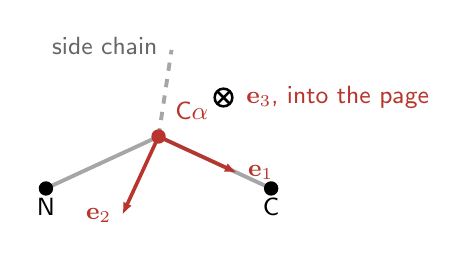
\begin{tikzpicture}[x=11mm, y=11mm]
  \coordinate (N) at (-1.3,-0.6); \coordinate (CA) at (0,0); \coordinate (C) at (1.3,-0.6);
  \draw[black!35, line width=1.4pt] (N) -- (CA) -- (C);
  \draw[black!35, line width=1.4pt, dashed] (CA) -- (0.15,1.0);
  \fill[black] (N) circle (2.6pt) node[below] {N};
  \fill[black] (C) circle (2.6pt) node[below] {C};
  \node[anchor=east, text=black!60] at (0.1,1.05) {side chain};
  \draw[ETHRed, line width=1.3pt, -{Latex[length=4.5pt]}] (CA) -- (-24.8:1.0) node[right] {$\mathbf e_1$};
  \draw[ETHRed, line width=1.3pt, -{Latex[length=4.5pt]}] (CA) -- (245.2:1.0) node[left] {$\mathbf e_2$};
  \fill[ETHRed] (CA) circle (2.6pt);
  \node[text=ETHRed, anchor=south west] at (0.08,0.08) {C$\alpha$};
  \belowpage{(0.75,0.45)}
  \node[text=ETHRed, anchor=west] at (0.9,0.45) {$\mathbf e_3$, into the page};
\end{tikzpicture}
\figcap{The backbone frame of one residue. $\mathbf e_1$ points to C, $\mathbf e_2$ is the N direction made orthogonal, $\mathbf e_3$ follows by the right-hand rule.}
\end{minipage}

\sect{evita}{2. IPA is invariant under rigid motions of the frames \si{SI 1.8.2, Algorithm 22, eqs.\ 3--6}}
Each residue $i$ has a frame $T_i$ and emits, per head $h$, query points $\vq_i^{hp}$ and key points $\vk_i^{hp}$ in its own frame. The attention logit (Algorithm 22, line 7) is
\[
a_{ij}^h=\operatorname{softmax}_j\!\Big(w_L\Big(\tfrac{1}{\sqrt c}\,\mathbf q_i^{h\top}\mathbf k_j^h + b_{ij}^h
-\tfrac{\gamma^h w_C}{2}\sum_p\big\|T_i\circ\vq_i^{hp}-T_j\circ\vk_j^{hp}\big\|^2\Big)\Big).
\]
Apply one rigid motion $\Tg$ to every frame. It cancels in the only geometric term, because the norm is invariant under rigid transforms, and again when the output points (line 10) are mapped back into frame $i$:
\[
\big\|(\Tg\circ T_i)\circ\vq_i^{hp}-(\Tg\circ T_j)\circ\vk_j^{hp}\big\|^2
=\big\|T_i\circ\vq_i^{hp}-T_j\circ\vk_j^{hp}\big\|^2, \qquad\si{eqs.\ 3, 4}
\]
\[
(\Tg\circ T_i)^{-1}\circ\sum_j a_{ij}^h\big((\Tg\circ T_j)\circ\vpt_j^{hp}\big)
=T_i^{-1}\circ\sum_j a_{ij}^h\big(T_j\circ\vpt_j^{hp}\big). \qquad\si{eqs.\ 5, 6}
\]
\begin{center}
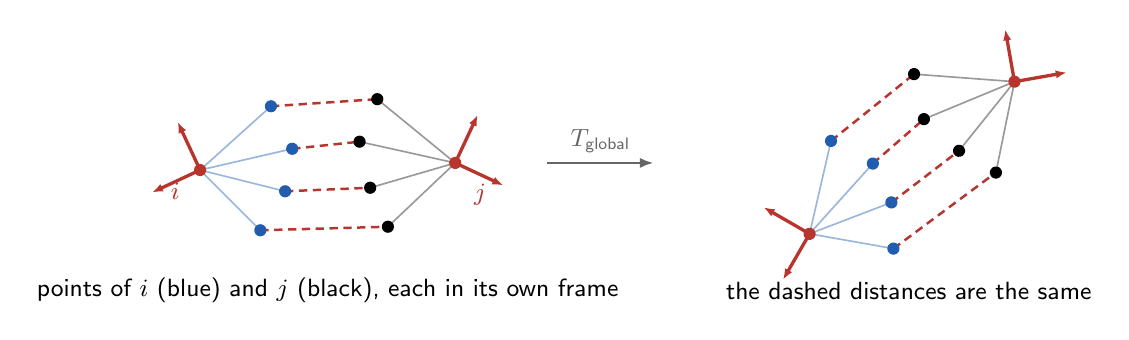
\begin{tikzpicture}[x=9mm, y=9mm]
  \ipapair
  \node[text=ETHRed] at (-0.35,-0.3) {$i$}; \node[text=ETHRed] at (3.95,-0.35) {$j$};
  \draw[black!60, line width=1pt, -{Latex[length=5pt]}] (4.9,0.1) -- (6.4,0.1) node[midway, above] {$\Tg$};
  \begin{scope}[shift={(8.6,-0.9)}, rotate=35]
    \ipapair
  \end{scope}
  \node at (1.8,-1.7) {points of $i$ (blue) and $j$ (black), each in its own frame};
  \node at (10.0,-1.7) {the dashed distances are the same};
\end{tikzpicture}
\figcap{The only geometry in IPA is the set of distances between points placed in the frames. A rigid motion of all frames moves the points together and leaves the distances unchanged, so the attention weights and the output are unchanged. Exact, by construction, not learned.}
\end{center}
A remark the SI does not make: the two cancellations use only $\|\Tg\circ\vx\|=\|\vx\|$, which also holds for reflections. IPA as a function of frames is invariant under all of $\E$. Chirality is not in IPA. It is in how frames are obtained from atoms (section 1) and in the loss (section 5).

\sect{evita}{3. The backbone update makes each block equivariant \si{SI 1.8, 1.8.3, Algorithm 23}}
\begin{minipage}[c]{0.55\textwidth}
From $\tilde{\mathbf s}_i$ alone the network predicts a quaternion $(1,b_i,c_i,d_i)$, normalised, and a translation, giving a small transform $T_i^{\text{upd}}$. The frame is updated in its own local coordinates,
\[
T_i\leftarrow T_i\circ T_i^{\text{upd}}. \qquad\si{Algorithm 20, line 10}
\]
If all frames are moved by $\Tg$, section 2 says $\tilde{\mathbf s}_i$ and hence $T_i^{\text{upd}}$ are unchanged, and
$(\Tg\circ T_i)\circ T_i^{\text{upd}}=\Tg\circ(T_i\circ T_i^{\text{upd}})$ by associativity. The output moves with the input: ``this update rule is equivariant under rigid motions'' \si{SI p.~28}. Eight such blocks with shared weights compose to an equivariant structure module.
\end{minipage}\hfill
\begin{minipage}[c]{0.42\textwidth}
\centering
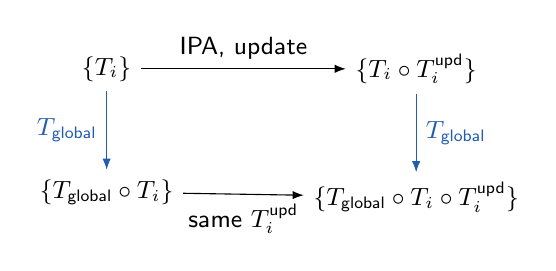
\begin{tikzpicture}[node distance=10mm and 26mm]
  \node (A) {$\{T_i\}$};
  \node[right=of A] (B) {$\{T_i\circ T_i^{\text{upd}}\}$};
  \node[below=of A] (C) {$\{\Tg\circ T_i\}$};
  \node[below=of B] (D) {$\{\Tg\circ T_i\circ T_i^{\text{upd}}\}$};
  \draw[-{Latex[length=4pt]}] (A) -- (B) node[midway, above] {IPA, update};
  \draw[-{Latex[length=4pt]}] (C) -- (D) node[midway, below] {same $T_i^{\text{upd}}$};
  \draw[-{Latex[length=4pt]}, ETHBlue] (A) -- (C) node[midway, left, text=ETHBlue] {$\Tg$};
  \draw[-{Latex[length=4pt]}, ETHBlue] (B) -- (D) node[midway, right, text=ETHBlue] {$\Tg$};
\end{tikzpicture}
\figcap{Equivariance is this square commuting: moving the frames first or last gives the same result, because the update is computed in local coordinates.}
\end{minipage}

Two facts that bound the claim. First, all frames start as the identity, the ``black hole initialization'' \si{SI 1.8, Algorithm 20 line 4}, so there is no input geometry at the start. Equivariance says the module never prefers a global frame. The global frame of the output is arbitrary, which is why the loss has to be invariant (section 5). Second, the Evoformer has no geometry at all. Recycling feeds the previous structure back only as binned C$\beta$ distances \si{SI 1.10, Algorithm 32}, which are invariant under all of $\E$, reflection included.

\sect{ben}{4. A reflection of the atoms is visible in local coordinates \si{SI 1.9.3, eqs.\ 10--15}}
\begin{minipage}[c]{0.55\textwidth}
Reflect every atom, $\vx\mapsto-\vx$. Rebuilding the frames with Algorithm 21 from the reflected atoms gives
\[
T_i=(R_i,\vt_i)\ \mapsto\ \Big(R_i\begin{pmatrix}-1&0&0\\0&-1&0\\0&0&1\end{pmatrix},\,-\vt_i\Big), \qquad\si{eq.\ 11}
\]
because $\mathbf e_1$ and $\mathbf e_2$ flip sign with the atoms while $\mathbf e_3=\mathbf e_1\times\mathbf e_2$ does not. The local coordinates of any atom then change by
\[
T_i^{-1}\circ\vx_j\ \mapsto\
\begin{pmatrix}1&0&0\\0&1&0\\0&0&-1\end{pmatrix}\big(T_i^{-1}\circ\vx_j\big). \qquad\si{eqs.\ 12--15}
\]
A reflection flips exactly the $z$ component of every local coordinate. Everything that works in local coordinates, IPA and FAPE, can therefore tell a protein from its mirror image.
\end{minipage}\hfill
\begin{minipage}[c]{0.42\textwidth}
\centering
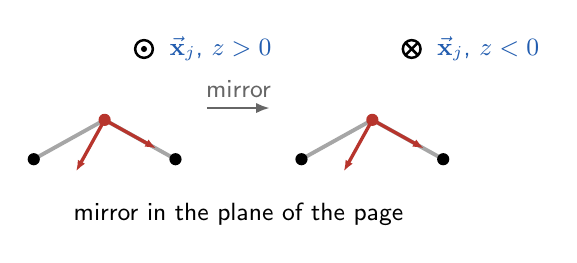
\begin{tikzpicture}[x=10mm, y=10mm]
  \foreach \dx/\sym/\lab in {0/abovepage/{$z>0$}, 3.4/belowpage/{$z<0$}} {
    \begin{scope}[shift={(\dx,0)}]
      \draw[black!35, line width=1.4pt] (-0.9,-0.5) -- (0,0) -- (0.9,-0.5);
      \fill[black] (-0.9,-0.5) circle (2.2pt); \fill[black] (0.9,-0.5) circle (2.2pt);
      \draw[ETHRed, line width=1.2pt, -{Latex[length=4pt]}] (0,0) -- (-29:0.75);
      \draw[ETHRed, line width=1.2pt, -{Latex[length=4pt]}] (0,0) -- (241:0.75);
      \fill[ETHRed] (0,0) circle (2.2pt);
      \csname\sym\endcsname{(0.5,0.9)}
      \node[anchor=west, text=ETHBlue] at (0.7,0.9) {$\vx_j$, \lab};
    \end{scope}
  }
  \draw[black!60, line width=1pt, -{Latex[length=5pt]}] (1.3,0.15) -- (2.1,0.15) node[midway, above] {mirror};
  \node at (1.7,-1.2) {mirror in the plane of the page};
\end{tikzpicture}
\figcap{Mirror the protein in the page. The three frame atoms lie in the page and stay, so the frame stays. An atom above the page ($\odot$) moves below it ($\otimes$): its local $z$ changes sign. Any mirror is this one up to a rotation, which the frames absorb.}
\end{minipage}

\sect{ben}{5. FAPE is invariant under rigid motions and sees chirality \si{SI 1.9.2, Algorithm 28, eqs.\ 16--17}}
For predicted frames and atoms $\{T_i\},\{\vx_j\}$ and the true $\{T_i^{\text{true}}\},\{\vx_j^{\text{true}}\}$,
\[
\vx_{ij}=T_i^{-1}\circ\vx_j,\qquad \vx_{ij}^{\text{true}}=T_i^{\text{true}\,-1}\circ\vx_j^{\text{true}},\qquad
d_{ij}=\sqrt{\|\vx_{ij}-\vx_{ij}^{\text{true}}\|^2+\epsilon},\qquad
\mathcal L_{\text{FAPE}}=\tfrac1Z\operatorname{mean}_{i,j}\big(\min(d_{\text{clamp}},d_{ij})\big),
\]
with $Z=d_{\text{clamp}}=10$\,\AA. Every atom is scored in every frame, $N_{\text{frames}}\times N_{\text{atoms}}$ terms.
\begin{center}
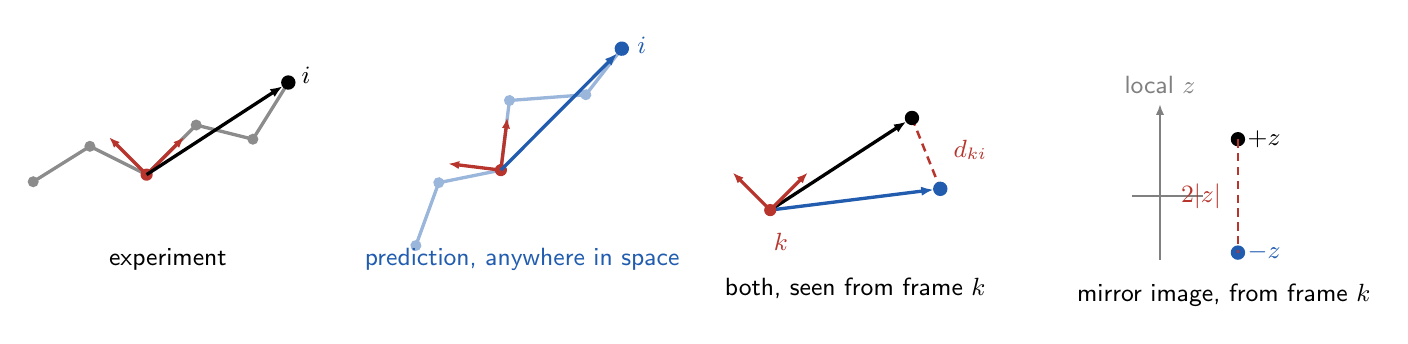
\begin{tikzpicture}[x=9mm, y=9mm]
  \begin{scope}
    \fapechain{black}{(3.1,0.6)}{(3.6,1.4)}{(0.25,0.1)}
    \node at (1.9,-1.1) {experiment};
  \end{scope}
  \begin{scope}[shift={(5.4,-0.9)}, rotate=38]
    \fapechain{ETHBlue}{(3.2,0.2)}{(4.0,0.4)}{(0.28,0.05)}
  \end{scope}
  \node[text=ETHBlue] at (6.9,-1.1) {prediction, anywhere in space};
  \begin{scope}[shift={(10.4,-0.4)}]
    \draw[black, line width=1.2pt, -{Latex[length=4.5pt]}, shorten >=2.4pt] (0,0) -- (2.0,1.3);
    \draw[ETHBlue, line width=1.2pt, -{Latex[length=4.5pt]}, shorten >=2.4pt] (0,0) -- (2.4,0.3);
    \draw[ETHRed, line width=0.9pt, densely dashed] (2.0,1.3) -- (2.4,0.3);
    \fill[black] (2.0,1.3) circle (2.6pt);
    \fill[ETHBlue] (2.4,0.3) circle (2.6pt);
    \frameaxes{(0,0)}{45}
    \node[text=ETHRed, anchor=west] at (2.45,0.85) {$d_{ki}$};
    \node[text=ETHRed] at (0.15,-0.45) {$k$};
  \end{scope}
  \node at (11.6,-1.5) {both, seen from frame $k$};
  \begin{scope}[shift={(15.9,-0.2)}]
    \draw[black!50, line width=0.8pt, -{Latex[length=4pt]}] (0,-0.9) -- (0,1.3) node[above] {local $z$};
    \draw[black!50, line width=0.8pt] (-0.4,0) -- (0.6,0);
    \fill[black] (1.1,0.8) circle (2.6pt) node[right] {$+z$};
    \fill[ETHBlue] (1.1,-0.8) circle (2.6pt) node[right] {$-z$};
    \draw[ETHRed, line width=0.9pt, densely dashed] (1.1,0.8) -- (1.1,-0.8);
    \node[text=ETHRed, anchor=east] at (1.0,0) {$2|z|$};
  \end{scope}
  \node at (16.8,-1.6) {mirror image, from frame $k$};
\end{tikzpicture}
\figcap{Left and middle: the prediction may sit anywhere, FAPE compares it with the experiment in the local frame $k$, so a rigid motion of the whole prediction changes nothing. Right: the mirror image has the same shape but, by section 4, every local $z$ flips, so each atom is off by $2|z|$ and the loss is large.}
\end{center}
Invariance: a rigid motion applied to the prediction moves $T_i$ and $\vx_j$ together, and $\vx_{ij}=T_i^{-1}\circ\vx_j$ is unchanged, by the same cancellation as in section 2. The same holds for the ground truth. So the loss ``will stay constant'' under any rotation and translation of either structure \si{SI p.~34}. Not invariance: by section 4,
\[
\mathrm{FAPE}(X,X_{\text{reflection}})=\sum_{ij}\Big\|T_i^{-1}\circ\vx_j-\begin{pmatrix}1&0&0\\0&1&0\\0&0&-1\end{pmatrix}\big(T_i^{-1}\circ\vx_j\big)\Big\|
=2\sum_{ij}\big|(T_i^{-1}\circ\vx_j)_z\big| , \qquad\si{eqs.\ 16, 17}
\]
``a large positive value outside of degenerate cases''. The ground truth frames come from the experimental atoms with the right-handed Algorithm 21, so the network is trained towards the correct hand.

\begin{minipage}[c]{0.6\textwidth}
Two further results. \si{SI 1.9.4, eqs.\ 18--22}: with $S$ the RMSD after the best alignment over $\SE$, $\mathrm{FAPE}(X,\tilde X)\ge S(\{\vx_j\},\{\tilde\vx_j\})$ regardless of the frames, so FAPE is zero only if the two point sets are related by a proper rigid motion, and a chiral pair always has positive loss, however the frames are built. \si{SI 1.9.5, eqs.\ 23--30}: idealised FAPE is a pseudometric, non-negative, symmetric, with the triangle inequality.

Evidence that this is what fixes the hand \si{SI 1.9.3, Suppl.\ Fig.\ 9}: a model trained with dRMSD, a loss that is reflection invariant, reaches good lDDT-C$\alpha$, which cannot see chirality, but its GDT is bimodal, and the low mode is the mirror image: $\overline{\text{GDT}}$, the GDT against the reflected target, is high exactly there. ``FAPE is the main component that ensures the correct chirality of predicted structures.'' Side chains add a second source: atoms are built from the frames and the predicted $\chi$ angles with ideal geometry, which ``will always generate a left-handed molecule'' \si{SI p.~35}, so the network cannot build the mirror image of a side chain at all.
\end{minipage}\hfill
\begin{minipage}[c]{0.37\textwidth}
\centering
\includegraphics[page=37, trim=145 490 150 48, clip, width=\linewidth]{_AF2-SI.pdf}
\figcap{Suppl.\ Fig.\ 9: a model trained with dRMSD instead of FAPE, 87 CASP14 domains. GDT splits into two modes. The low mode scores high against the mirrored target ($\overline{\text{GDT}}$). lDDT-C$\alpha$ cannot see the difference.}
\end{minipage}

\sect{black}{6. Summary}
\smallskip
{\centering
\begin{tabular}{@{}llll@{}}
\toprule
Component & Under rigid motions, $\SE$ & Under reflection & Source \\
\midrule
Evoformer, recycling & no geometry, distances invariant & invariant & SI 1.10 \\
Frames from atoms & move with the atoms & do not reflect, eq.\ 11 & SI 1.8.1, 1.9.3 \\
IPA & invariant, exact & invariant, given the frames & SI 1.8.2 \\
Backbone update, one block & equivariant, exact & as the frames & SI 1.8.3 \\
FAPE & invariant & not invariant, eq.\ 17 & SI 1.9.2, 1.9.3 \\
All-atom construction & equivariant & always the correct hand & SI 1.8.4, p.~35 \\
\bottomrule
\end{tabular}\par}
\smallskip

What to say if asked ``is it SE(3)-equivariant'': yes, the structure module is exactly equivariant under rotations and translations and the loss is invariant, both by working in local frames. It is deliberately not equivariant under reflections, so the output has a definite handedness, learned from the data. What not to say: that AlphaFold uses equivariant kernels or spherical harmonics as in SE(3)-Transformers. The mechanism is only that points are expressed in per-residue frames, so a global motion cancels. The SI proves this in four lines, equations 3 to 6.

\end{document}
